\documentclass[12pt]{article}
\usepackage{amsmath, amssymb, amsthm}
\usepackage{geometry}
\usepackage{hyperref}
\usepackage{listings}
\usepackage{xcolor}
\usepackage{graphicx}
\usepackage{booktabs}
\usepackage{array}
\usepackage{tabularx}
\usepackage{placeins}
\usepackage{tikz}
\usetikzlibrary{arrows.meta, positioning}
\definecolor{stageblue}{HTML}{307BF3}

\geometry{margin=1in}

\lstset{
    language=Python,
    basicstyle=\ttfamily\small,
    keywordstyle=\color{blue},
    stringstyle=\color{red},
    commentstyle=\color{green!50!black},
    showstringspaces=false,
    breaklines=true,
    frame=single,
    numbers=left,
    numberstyle=\tiny
}

\title{Special Topics in Applied Mathematics I \\ Solution 2}
\author{XIA JIAHAN}
\date{\today}

\begin{document}
\maketitle

\section{Introduction to Recommendation Systems}

In the information explosion era, recommendation systems (RS) are essential for filtering vast data and delivering personalized content across platforms like Amazon, Netflix, YouTube, and social media, enhancing user experience and business value by predicting preferences. They use machine learning to model similarities between items and user interests, powering two main types of suggestions: personalized homepage feeds (unique to each user) and related item recommendations (e.g., suggesting science apps when viewing a math app). This enables platforms like YouTube and the Google Play Store to anticipate what to show next. The core motivation is to help users navigate immense content libraries, where search alone falls short, by surfacing relevant, sometimes unexpected items and facilitating discovery.

A recommender system matches a user's query (context) to recommendable entities (items) by learning embeddings that place queries and items in a shared vector space for efficient similarity computation. It then performs candidate generation to quickly narrow a huge corpus to hundreds or thousands of candidates, scoring to rank this smaller set and select roughly ten items to display, and finally re-ranking to apply constraints such as removing content the user dislikes, boosting fresher items, and ensuring diversity and fairness. We will discuss each stage with examples from systems like YouTube.

\begin{figure}[htbp]
    \centering
    \resizebox{\linewidth}{!}{%
    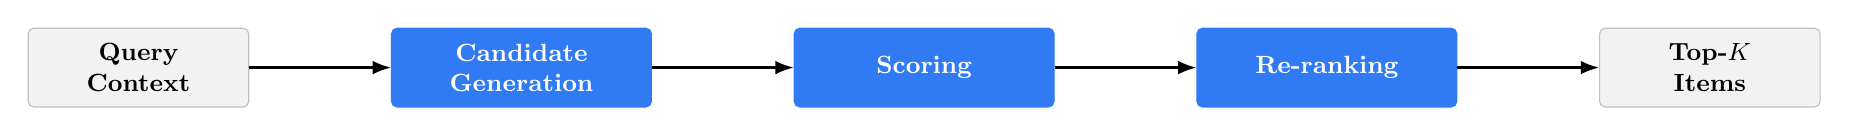
\begin{tikzpicture}[
        node distance=1.8cm,
        >=Latex,
        stage/.style={draw=stageblue, fill=stageblue, rounded corners=2pt, text=white, font=\small\bfseries, minimum height=10mm, minimum width=33mm, align=center},
        io/.style={draw=black!25, fill=black!5, rounded corners=2pt, font=\small\bfseries, minimum height=10mm, minimum width=28mm, align=center}
    ]
        \node[io] (query) {Query\\Context};
        \node[stage, right=of query] (cand) {Candidate\\Generation};
        \node[stage, right=of cand] (score) {Scoring};
        \node[stage, right=of score] (rerank) {Re-ranking};
        \node[io, right=of rerank] (results) {Top-$K$\\Items};

        \draw[->, thick] (query) -- (cand);
        \draw[->, thick] (cand) -- (score);
        \draw[->, thick] (score) -- (rerank);
        \draw[->, thick] (rerank) -- (results);
    \end{tikzpicture}%
    }
    \caption{Overview of the Recommender System Process}
    \label{fig:process_flow}
\end{figure}

\section{Candidate generation overview}
Candidate generation is the first stage of recommendation. Given a query, the system generates a set of relevant candidates. The following table shows two common candidate generation approaches:

\begin{table}[ht]
    \centering
    \renewcommand{\arraystretch}{1.2}
    \begin{tabularx}{\linewidth}{l X X}
        \toprule
        Type & Definition & Example \\
        \midrule
        content-based filtering & Uses \emph{similarity between items} to recommend items similar to what the user likes. & If user A watches two cute cat videos, then the system can recommend cute animal videos to that user. \\
        \midrule
        collaborative filtering & Uses \emph{similarities between queries and items simultaneously} to provide recommendations. & If user A is similar to user B, and user B likes video 1, then the system can recommend video 1 to user A (even if user A hasn't seen any videos similar to video 1). \\
        \bottomrule
    \end{tabularx}
\end{table}

Both content-based and collaborative filtering embed items and queries (contexts) into a shared low-dimensional space \(E=\mathbb{R}^{d}\). Candidate generation then retrieves items whose embeddings are most similar to the query embedding: a similarity function \(s:E\times E\to\mathbb{R}\) ranks candidates by \(s(q,x)\). Common choices include cosine similarity, dot product, and Euclidean distance.

Unlike cosine similarity, dot product is sensitive to embedding norms, so large-norm vectors can be preferred even when the angle is similar. This can affect recommendations as follows:
\begin{itemize}
    \item Popular items often get large norms, so dot product can capture popularity but may cause popular items to dominate. A tempered variant is \(s(q,x)=\lVert q\rVert^{\alpha}\,\lVert x\rVert^{\alpha}\,\cos(q,x)\) for \(\alpha\in(0,1)\).
    \item Rare items may be updated infrequently; if initialized with large norms they can be over-recommended. To avoid this problem, be careful about embedding initialization and use appropriate regularization.
\end{itemize}

\section{Content-based filtering}

Content-based filtering recommends items that are similar to what a user already likes by comparing item feature vectors. Figure~\ref{fig:matrix1} illustrates a simple (binary) feature matrix for apps; a user can be represented in the same feature space using explicit preferences and past installs. Given a similarity metric (e.g., dot product), the system scores each candidate item against the user vector and recommends the highest-scoring items, without using information from other users.

\begin{figure}[htbp]
    \centering
    \includegraphics[width=0.8\linewidth]{Matrix1.png}
    \caption{A toy feature matrix for apps (rows) and features (columns).}
    \label{fig:matrix1}
\end{figure}
\FloatBarrier

Content-based filtering has the advantage that it does not require data about other users, since recommendations are computed specifically for a given user, which makes it easier to scale to a large user base; it can also capture a user’s particular interests and recommend niche items that few other users care about. However, it often relies on partially hand-engineered item features and substantial domain knowledge, so performance is limited by the quality of those features, and it can only recommend based on the user’s existing interests, giving it limited ability to broaden the user’s preferences beyond what they have already shown.

\section{Collaborative filtering}
To address some of the limitations of content-based filtering, collaborative filtering uses similarities between users and items simultaneously to provide recommendations. This allows for serendipitous recommendations; that is, collaborative filtering models can recommend an item to user A based on the interests of a similar user B. Furthermore, the embeddings can be learned automatically, without relying on hand-engineering of features.

Consider a movie recommendation system in which the training data consist of a feedback matrix in which:
\begin{itemize}
    \item Each row represents a user.
    \item Each column represents an item (a movie).
\end{itemize}

The feedback about movies falls into one of two categories:
\begin{itemize}
    \item \textbf{Explicit}---users specify how much they liked a particular movie by providing a numerical rating.
    \item \textbf{Implicit}---if a user watches a movie, the system infers that the user is interested.
\end{itemize}

To simplify, we assume that the feedback matrix is binary; that is, a value of \(1\) indicates interest in the movie. When a user visits the homepage, the system should recommend movies based on both:
\begin{itemize}
    \item similarity to movies the user has liked in the past;
    \item movies that similar users liked.
\end{itemize}

For the sake of illustration, let's hand-engineer some features for the movies described in the following table:

\begin{table}[ht]
    \centering
    \renewcommand{\arraystretch}{1.15}
    \begin{tabularx}{\linewidth}{>{\raggedright\arraybackslash}p{0.25\linewidth} c X}
        \toprule
        Movie & Rating & Description \\
        \midrule
        The Dark Knight Rises & PG-13 & Batman endeavors to save Gotham City from nuclear annihilation in this sequel to \emph{The Dark Knight}, set in the DC Comics universe. \\
        \midrule
        Harry Potter and the Sorcerer's Stone & PG & An orphaned boy discovers he is a wizard and enrolls in Hogwarts School of Witchcraft and Wizardry, where he wages his first battle against the evil Lord Voldemort. \\
        \midrule
        Shrek & PG & A lovable ogre and his donkey sidekick set off on a mission to rescue Princess Fiona, who is imprisoned in her castle by a dragon. \\
        \midrule
        The Triplets of Belleville & PG-13 & When professional cyclist Champion is kidnapped during the Tour de France, his grandmother and overweight dog journey overseas to rescue him, with the help of a trio of elderly jazz singers. \\
        \midrule
        Memento & R & An amnesiac desperately seeks to solve his wife's murder by tattooing clues onto his body. \\
        \bottomrule
    \end{tabularx}
\end{table}
\FloatBarrier


\end{document}

